\documentclass[11pt]{beamer}

\usetheme[progressbar=frametitle]{metropolis}
\usepackage{appendixnumberbeamer}
\usepackage{FiraSans}
\usepackage{graphicx} 
\usepackage{booktabs}
\usepackage[scale=2]{ccicons}
\usepackage{adjustbox}
\usepackage{soul}
\usepackage{caption}
	\captionsetup[figure]{	labelformat=empty, 
					font=scriptsize,
					labelfont=scriptsize, 
					justification=raggedleft}

\usepackage{pgfplots}
\usepgfplotslibrary{dateplot}



\usepackage{xspace}
\newcommand{\themename}{\textbf{\textsc{metropolis}}\xspace}

\title{Barriers to a summer fire regime in northern prairies }
\subtitle{Ecological, physical, and social}
\date{}
\author{Devan Allen McGranahan } 
\institute{\emph{Research Rangeland Management Scientist\textemdash Ecologist} \\
		     USDA Agricultural Research Service \\ 
	    	     Miles City, Montana}
    	   
		
\newcommand\blfootnotetext[1]{%
  \begingroup
  \renewcommand\thefootnote{}\footnote{#1}%
  \addtocounter{footnote}{-1}%
  \endgroup
}


\begin{document}

\maketitle

\begin{frame}{The Western fire regime concept } 
	\begin{center}
		\begin{figure}
			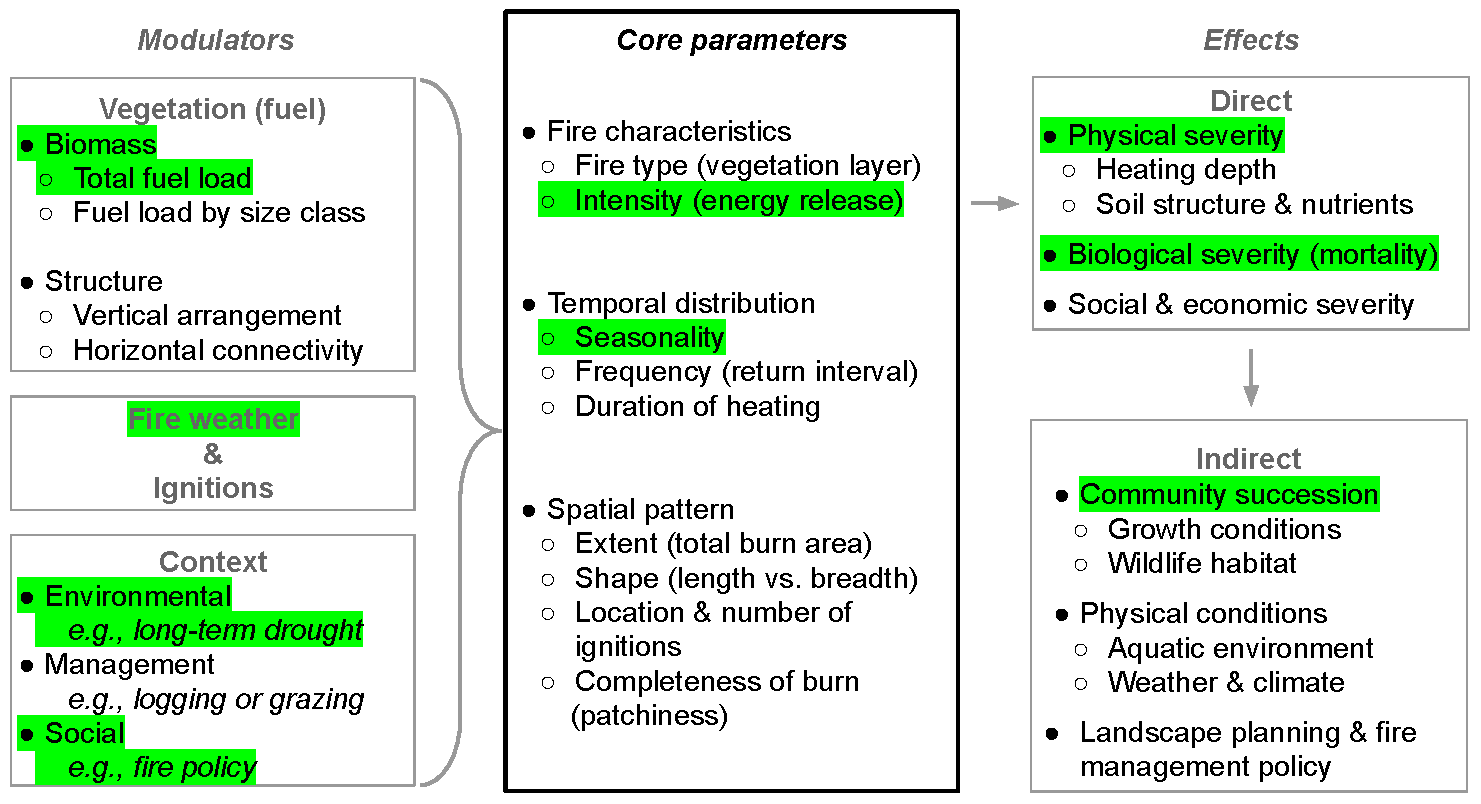
\includegraphics[width=1\linewidth]{figs/FireRegimeNAPC} 
		\end{figure}
	\end{center}
\end{frame}

\begin{frame}{The Western fire regime concept}
	\begin{center}
		\begin{figure}
			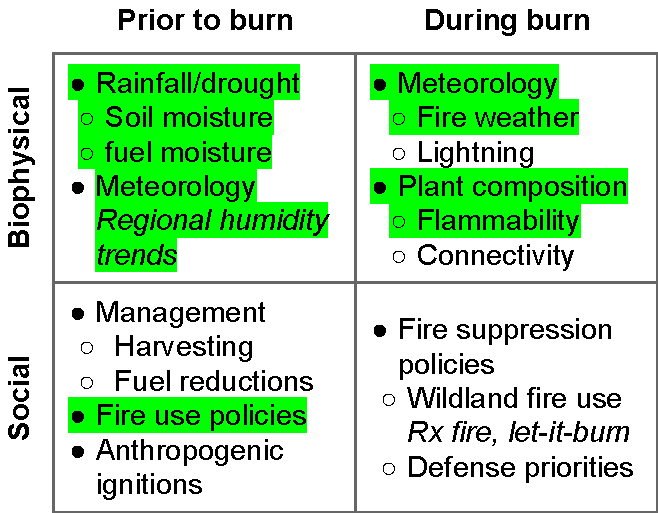
\includegraphics[width=0.9\linewidth]{figs/FireRegimeModulatorsNAPC} 
		\end{figure}
	\end{center}
\end{frame}


\begin{frame}{Rx fire in the Northern Great Plains}
	\begin{center}
		\begin{figure}
			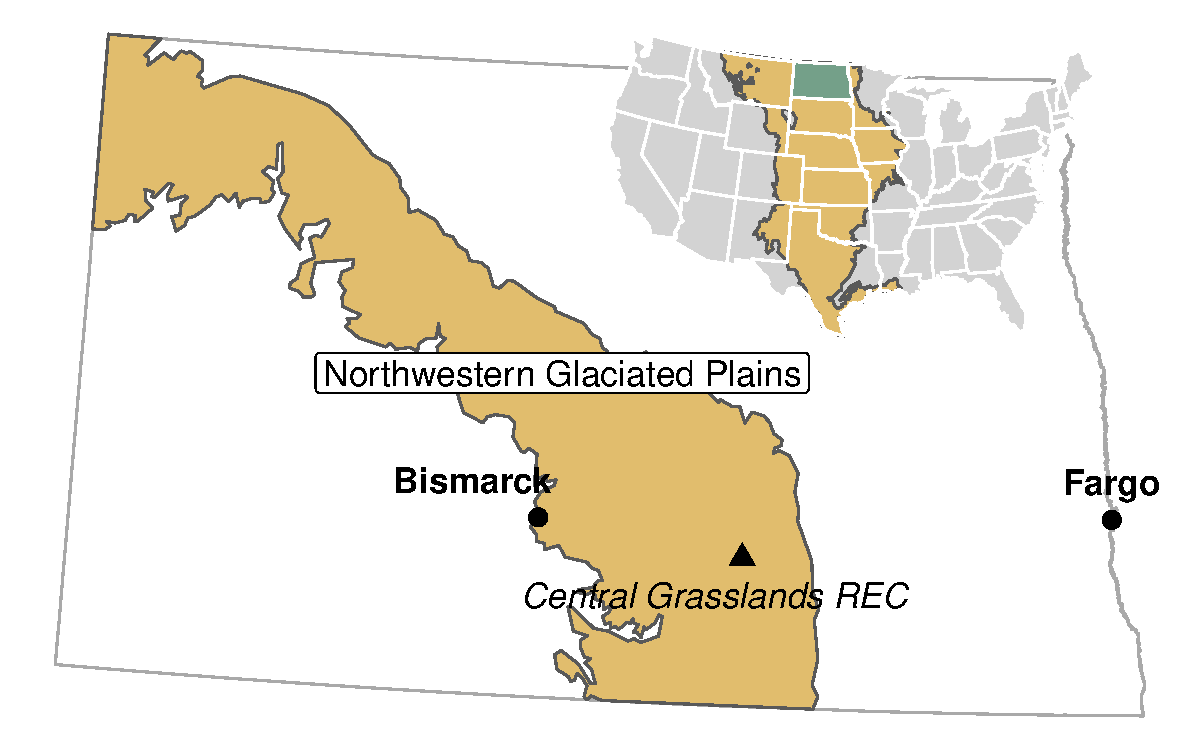
\includegraphics[width=1\linewidth]{figs/region_map-1.pdf} 
		\end{figure}
	\end{center}
\end{frame}

\begin{frame}{Rx fire in the Northern Great Plains}
	\begin{center}
		\begin{figure}
			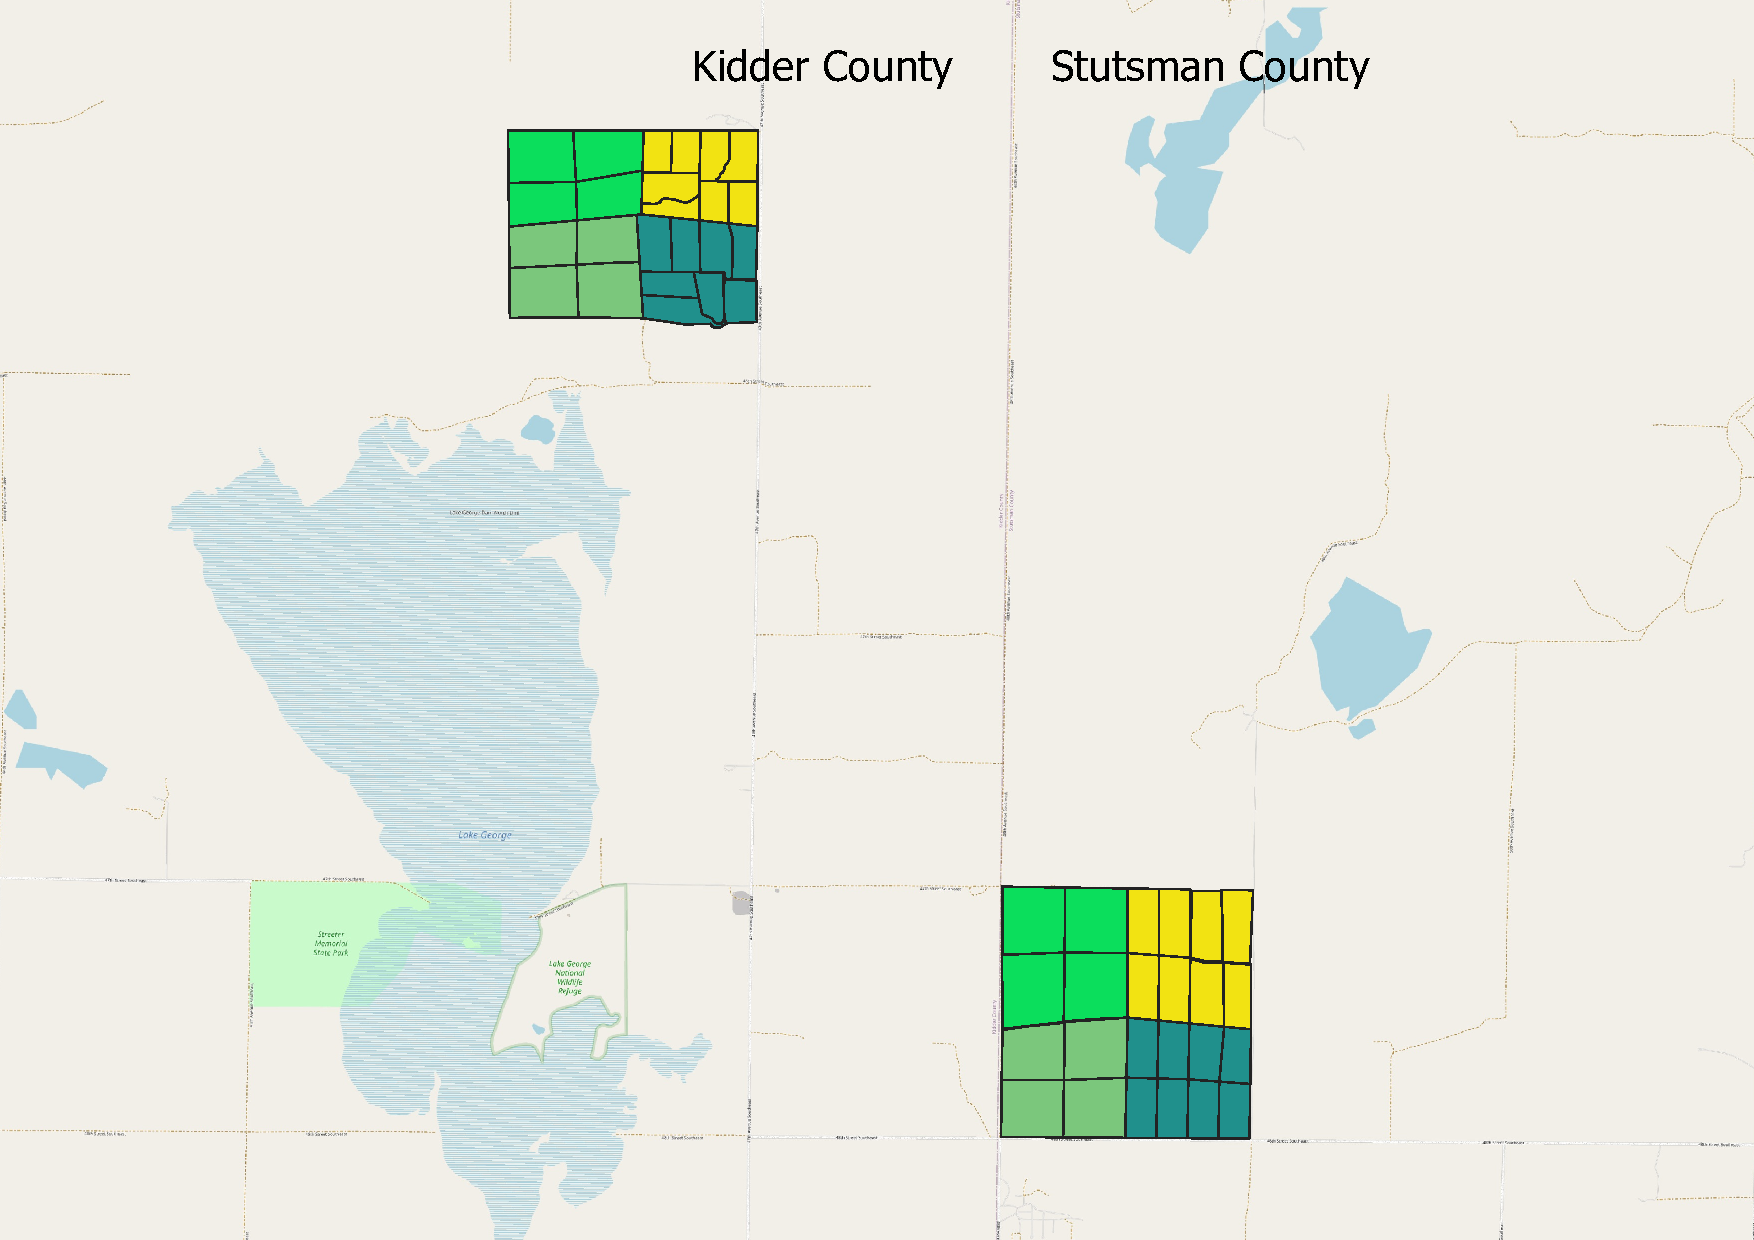
\includegraphics[width=1\linewidth]{figs/PBGmaps} 
		\end{figure}
	\end{center}
\end{frame}

\begin{frame}{Burns visible from space}
	\begin{center}
		\begin{figure}
			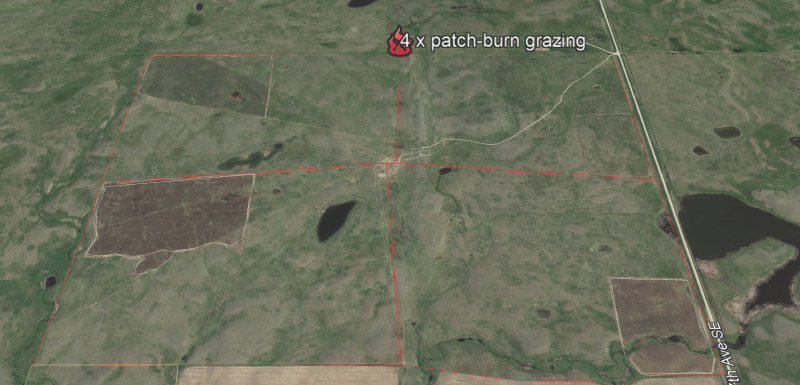
\includegraphics[width=1\linewidth]{figs/BobSWBurnedOutline2} 
		\end{figure}
	\end{center}
\end{frame}

\begin{frame}{Spotty success in completing summer burns}

	\begin{center}
		\begin{figure}
			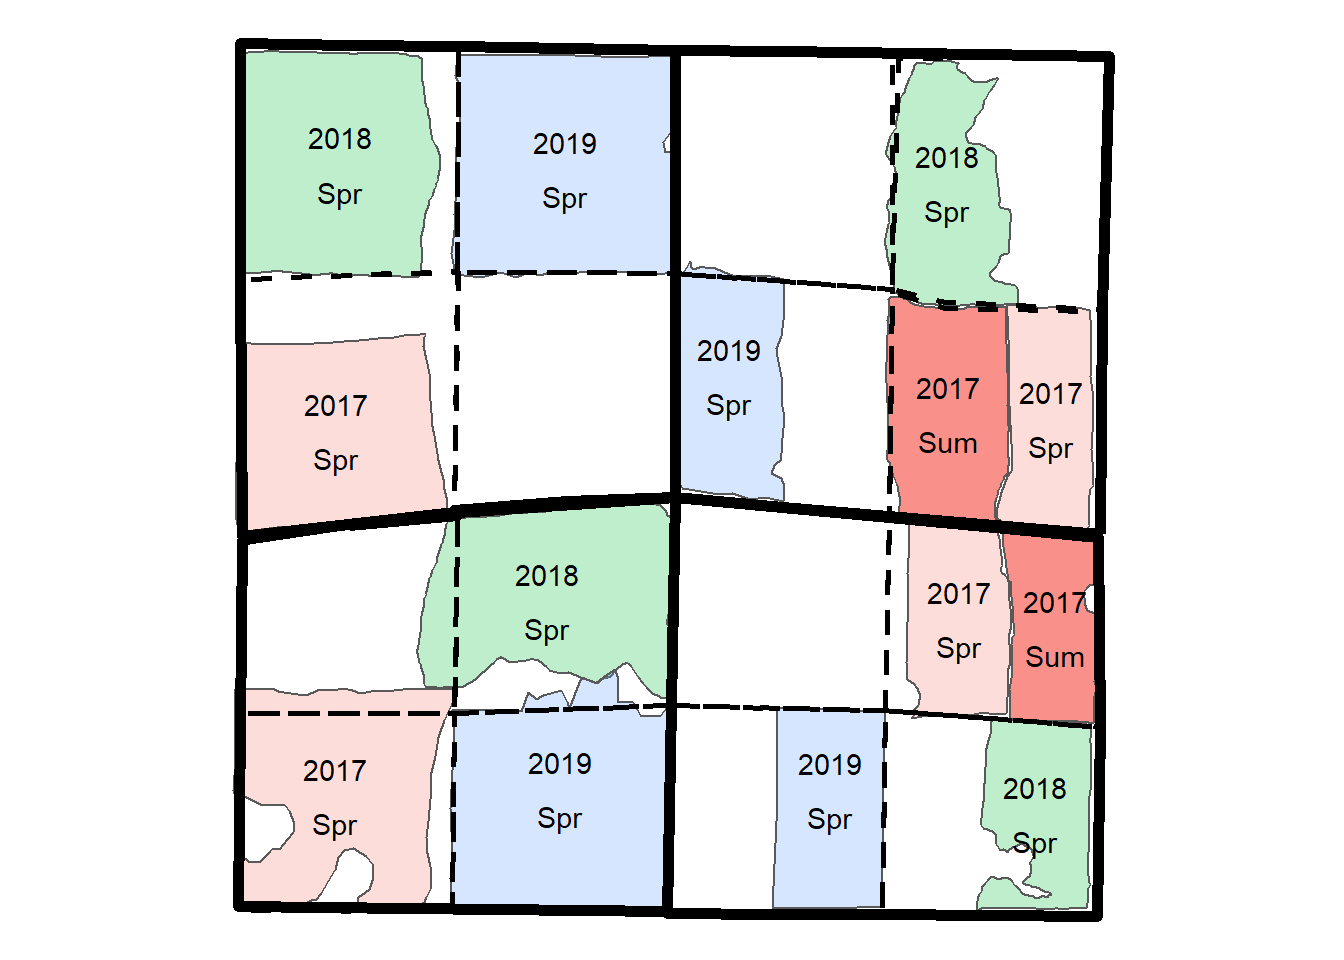
\includegraphics[width=0.9\linewidth]{figs/BarkerBurns-1} 
			\caption{2019 burn map for southern study block}
		\end{figure}
	\end{center}
\end{frame}

\section{A tale of two fires}

\begin{frame}{What a difference a few days makes! } 
	\begin{columns}
		\begin{column}{0.5\textwidth}
				\begin{center}
				\begin{figure}
					%\caption{5 May 2018}
					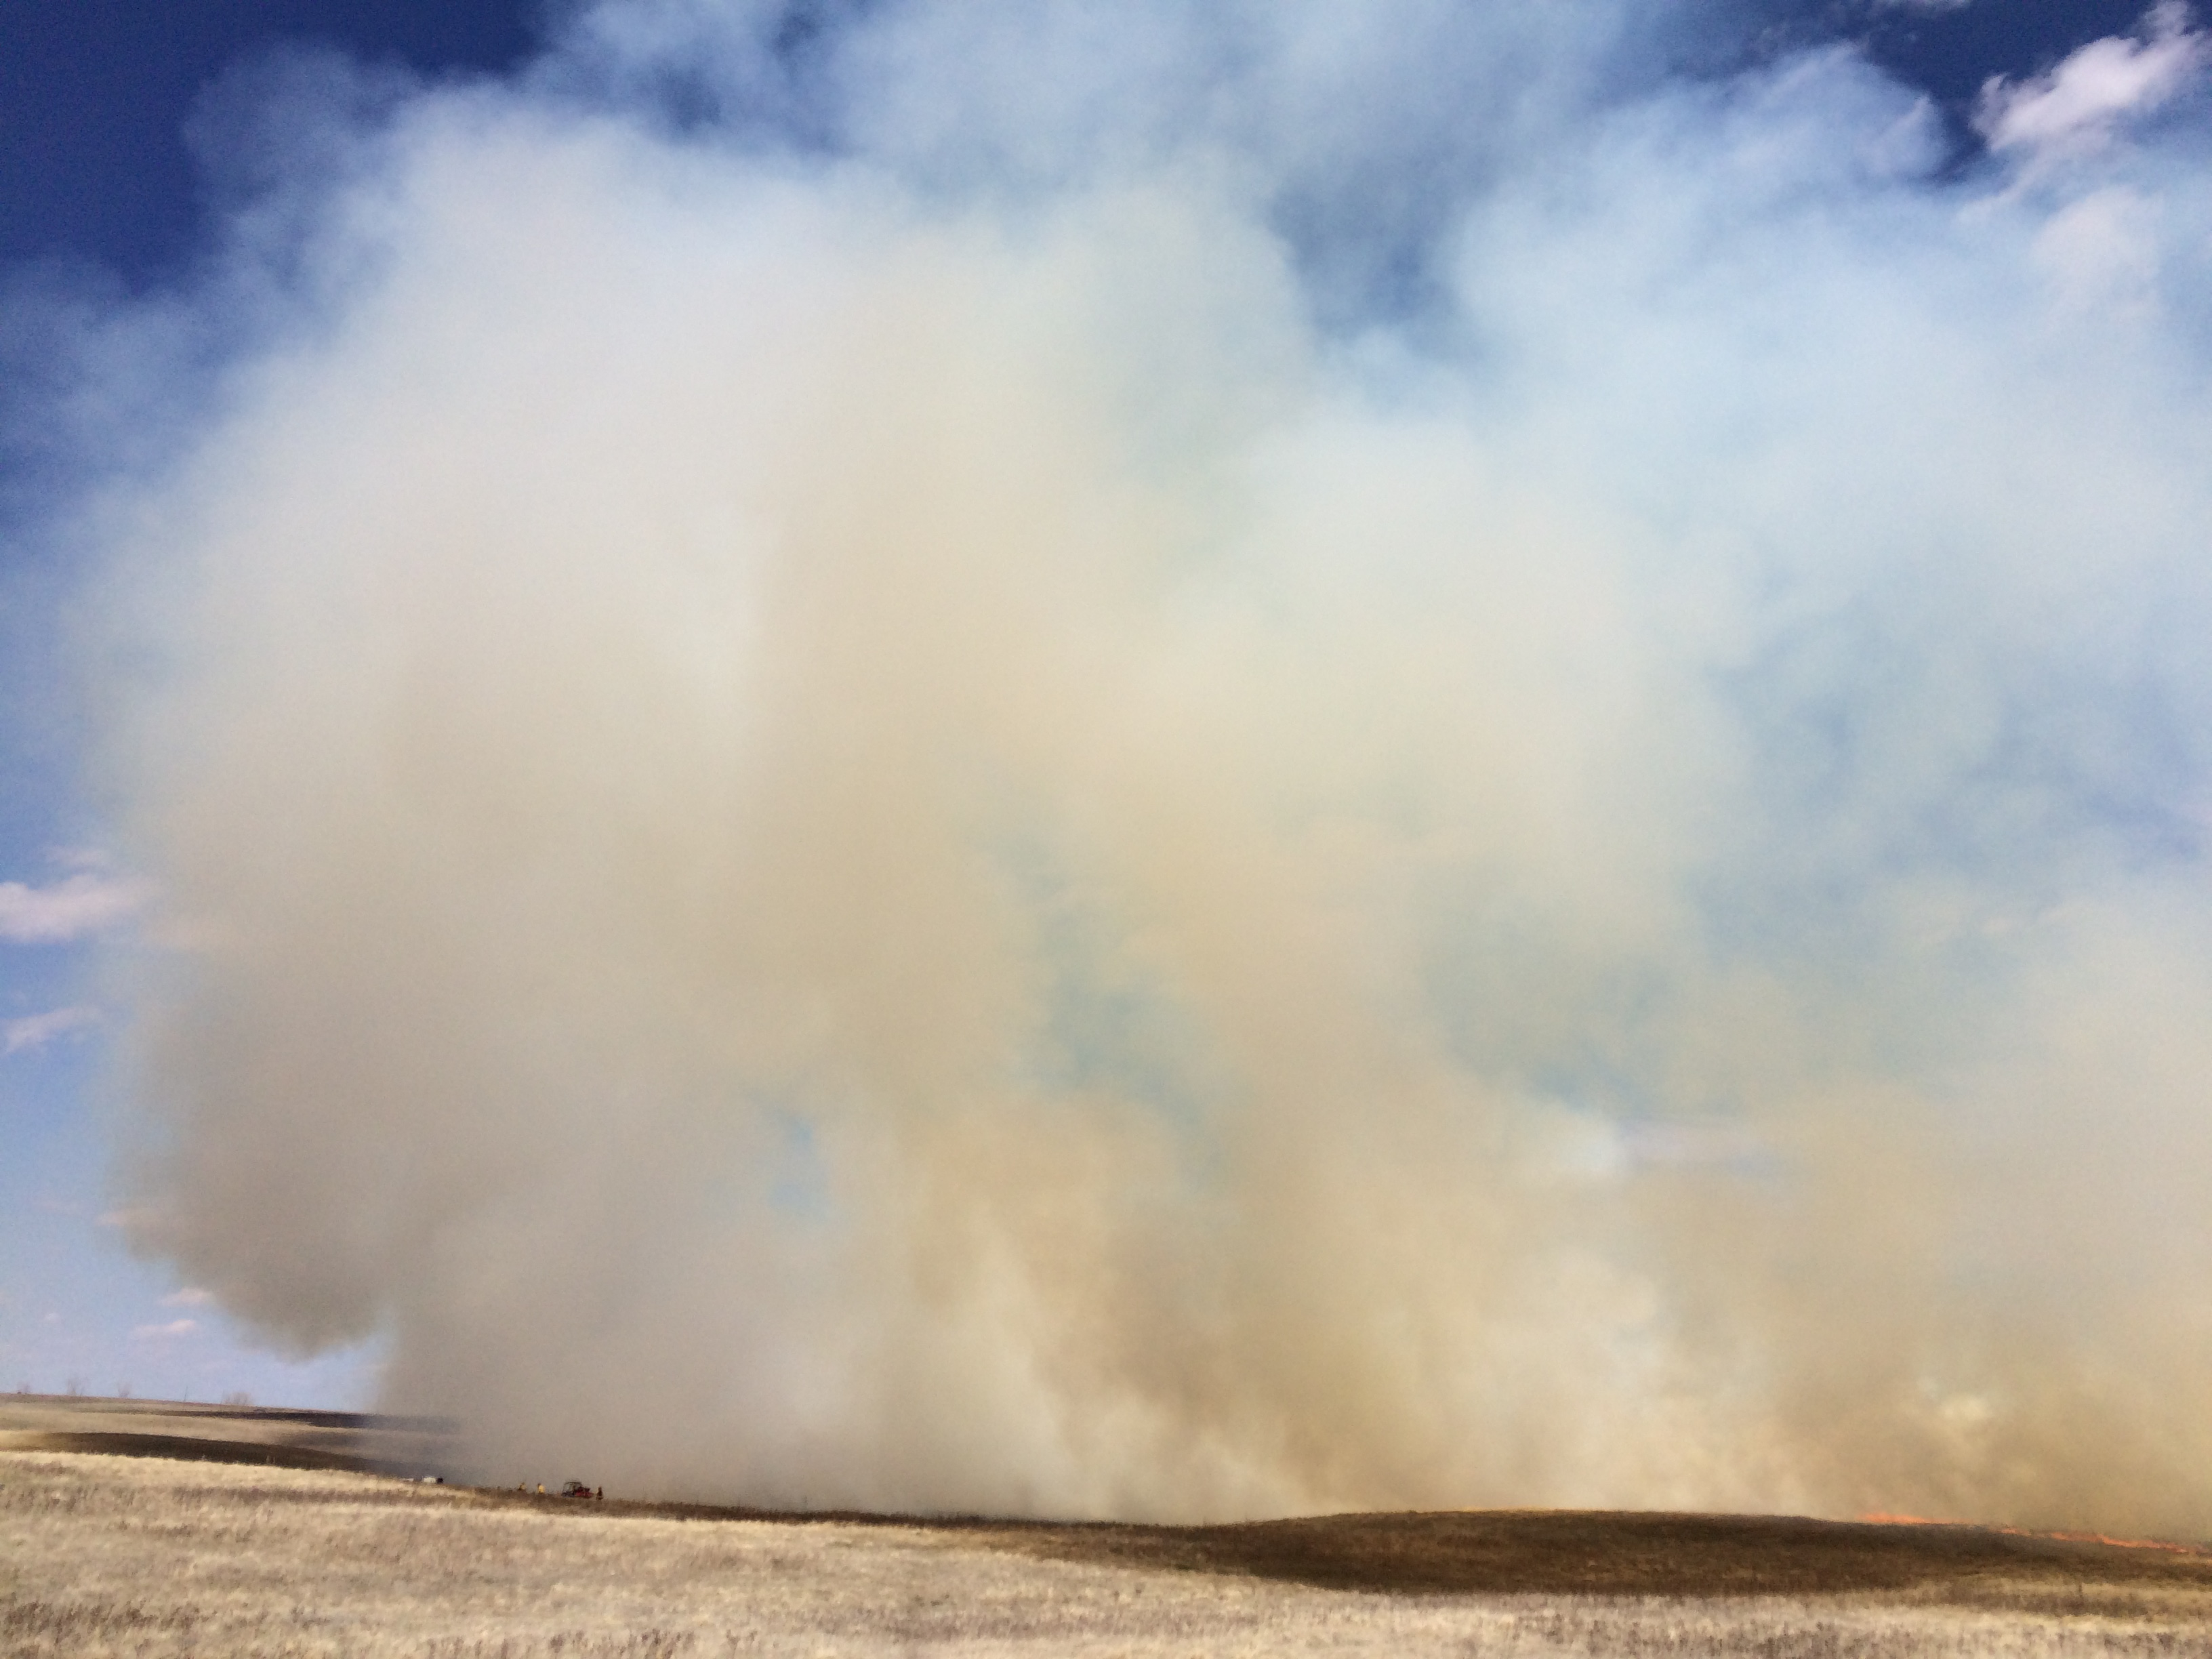
\includegraphics[width=0.9\linewidth]{figs/GoodBurn} 
				\end{figure}
			\end{center}
		\end{column}
		\begin{column}{0.5\textwidth}  
			\begin{center}
				\begin{figure}
					%\caption{16 May 2018}
					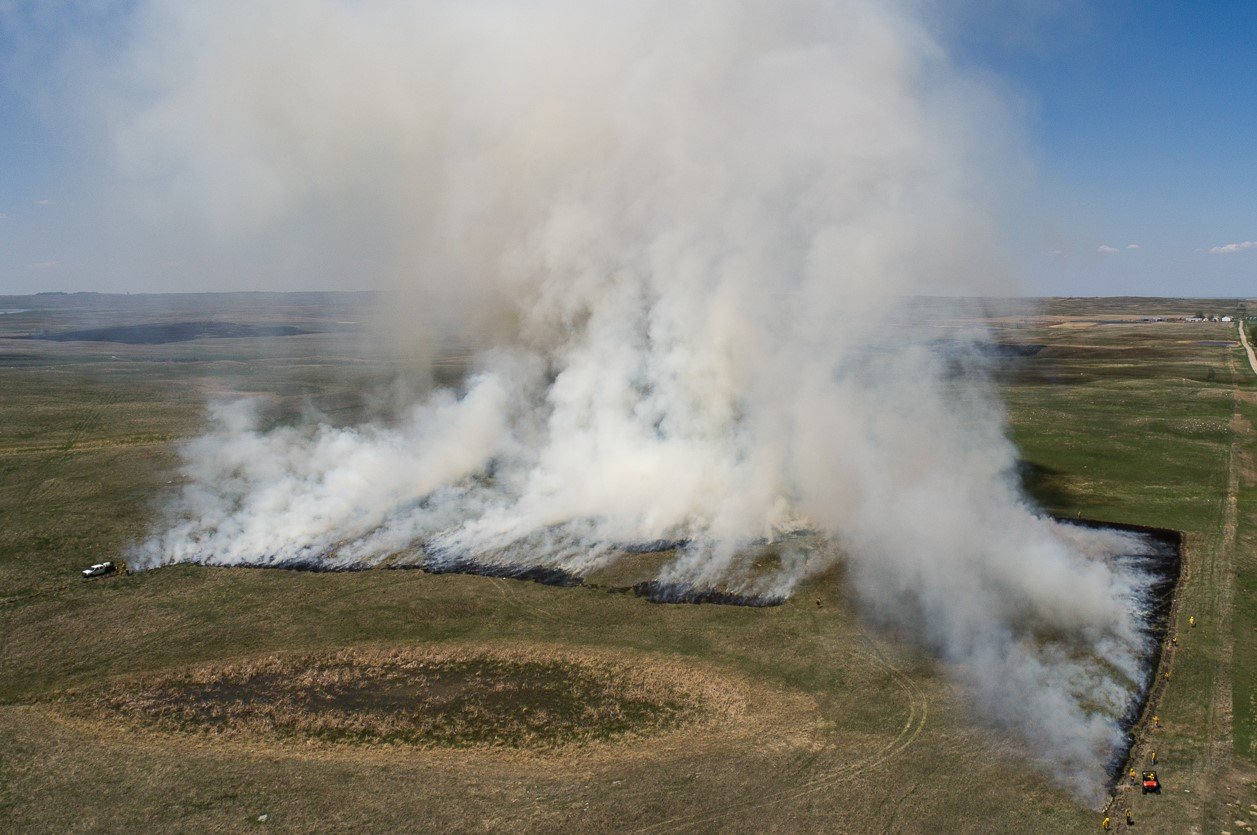
\includegraphics[width=1\linewidth]{figs/StreeterFire_17}  
				\end{figure}
			\end{center}
		\end{column}
	\end{columns}
\centering
\adjustbox{max height=\dimexpr\textheight-5.5cm\relax,
	max width=1\textwidth}{
	\begin{tabular}{ccc}
		\toprule
		5 May 2018 & \textbf{Date} & 16 May 2018 \\
		Weather & \textbf{Wind} & \\
		Fuels & \textbf{RH} & Yes \\ \bottomrule
	\end{tabular}
}
\end{frame}

\begin{frame}{Barriers to summer Rx fire } 
	All opportunities and limitations fit within fire regime concept
	\begin{itemize}
		\item Biophysical 
		\item[] \emph{mostly, \alert{too wet}}
		\begin{itemize}
			\item High live moisture fuel content (\emph{photosynthesis})
			\item High dead moisture fuel content (\emph{humidity})
			\item Poor convection/smoke dispersal (\emph{humidity})
		\end{itemize}
	\item[]
		\item Social 
		\item[] \emph{mostly, \alert{too dry}}
		\begin{itemize}
			\item Local burn restrictions
			\item Control issues
			\end{itemize}
	\end{itemize}

\end{frame}

\section{Biophysical barriers}

\section{Social barriers}

\begin{frame}{County-level burn restrictions}
	\begin{center}
		\begin{figure}
			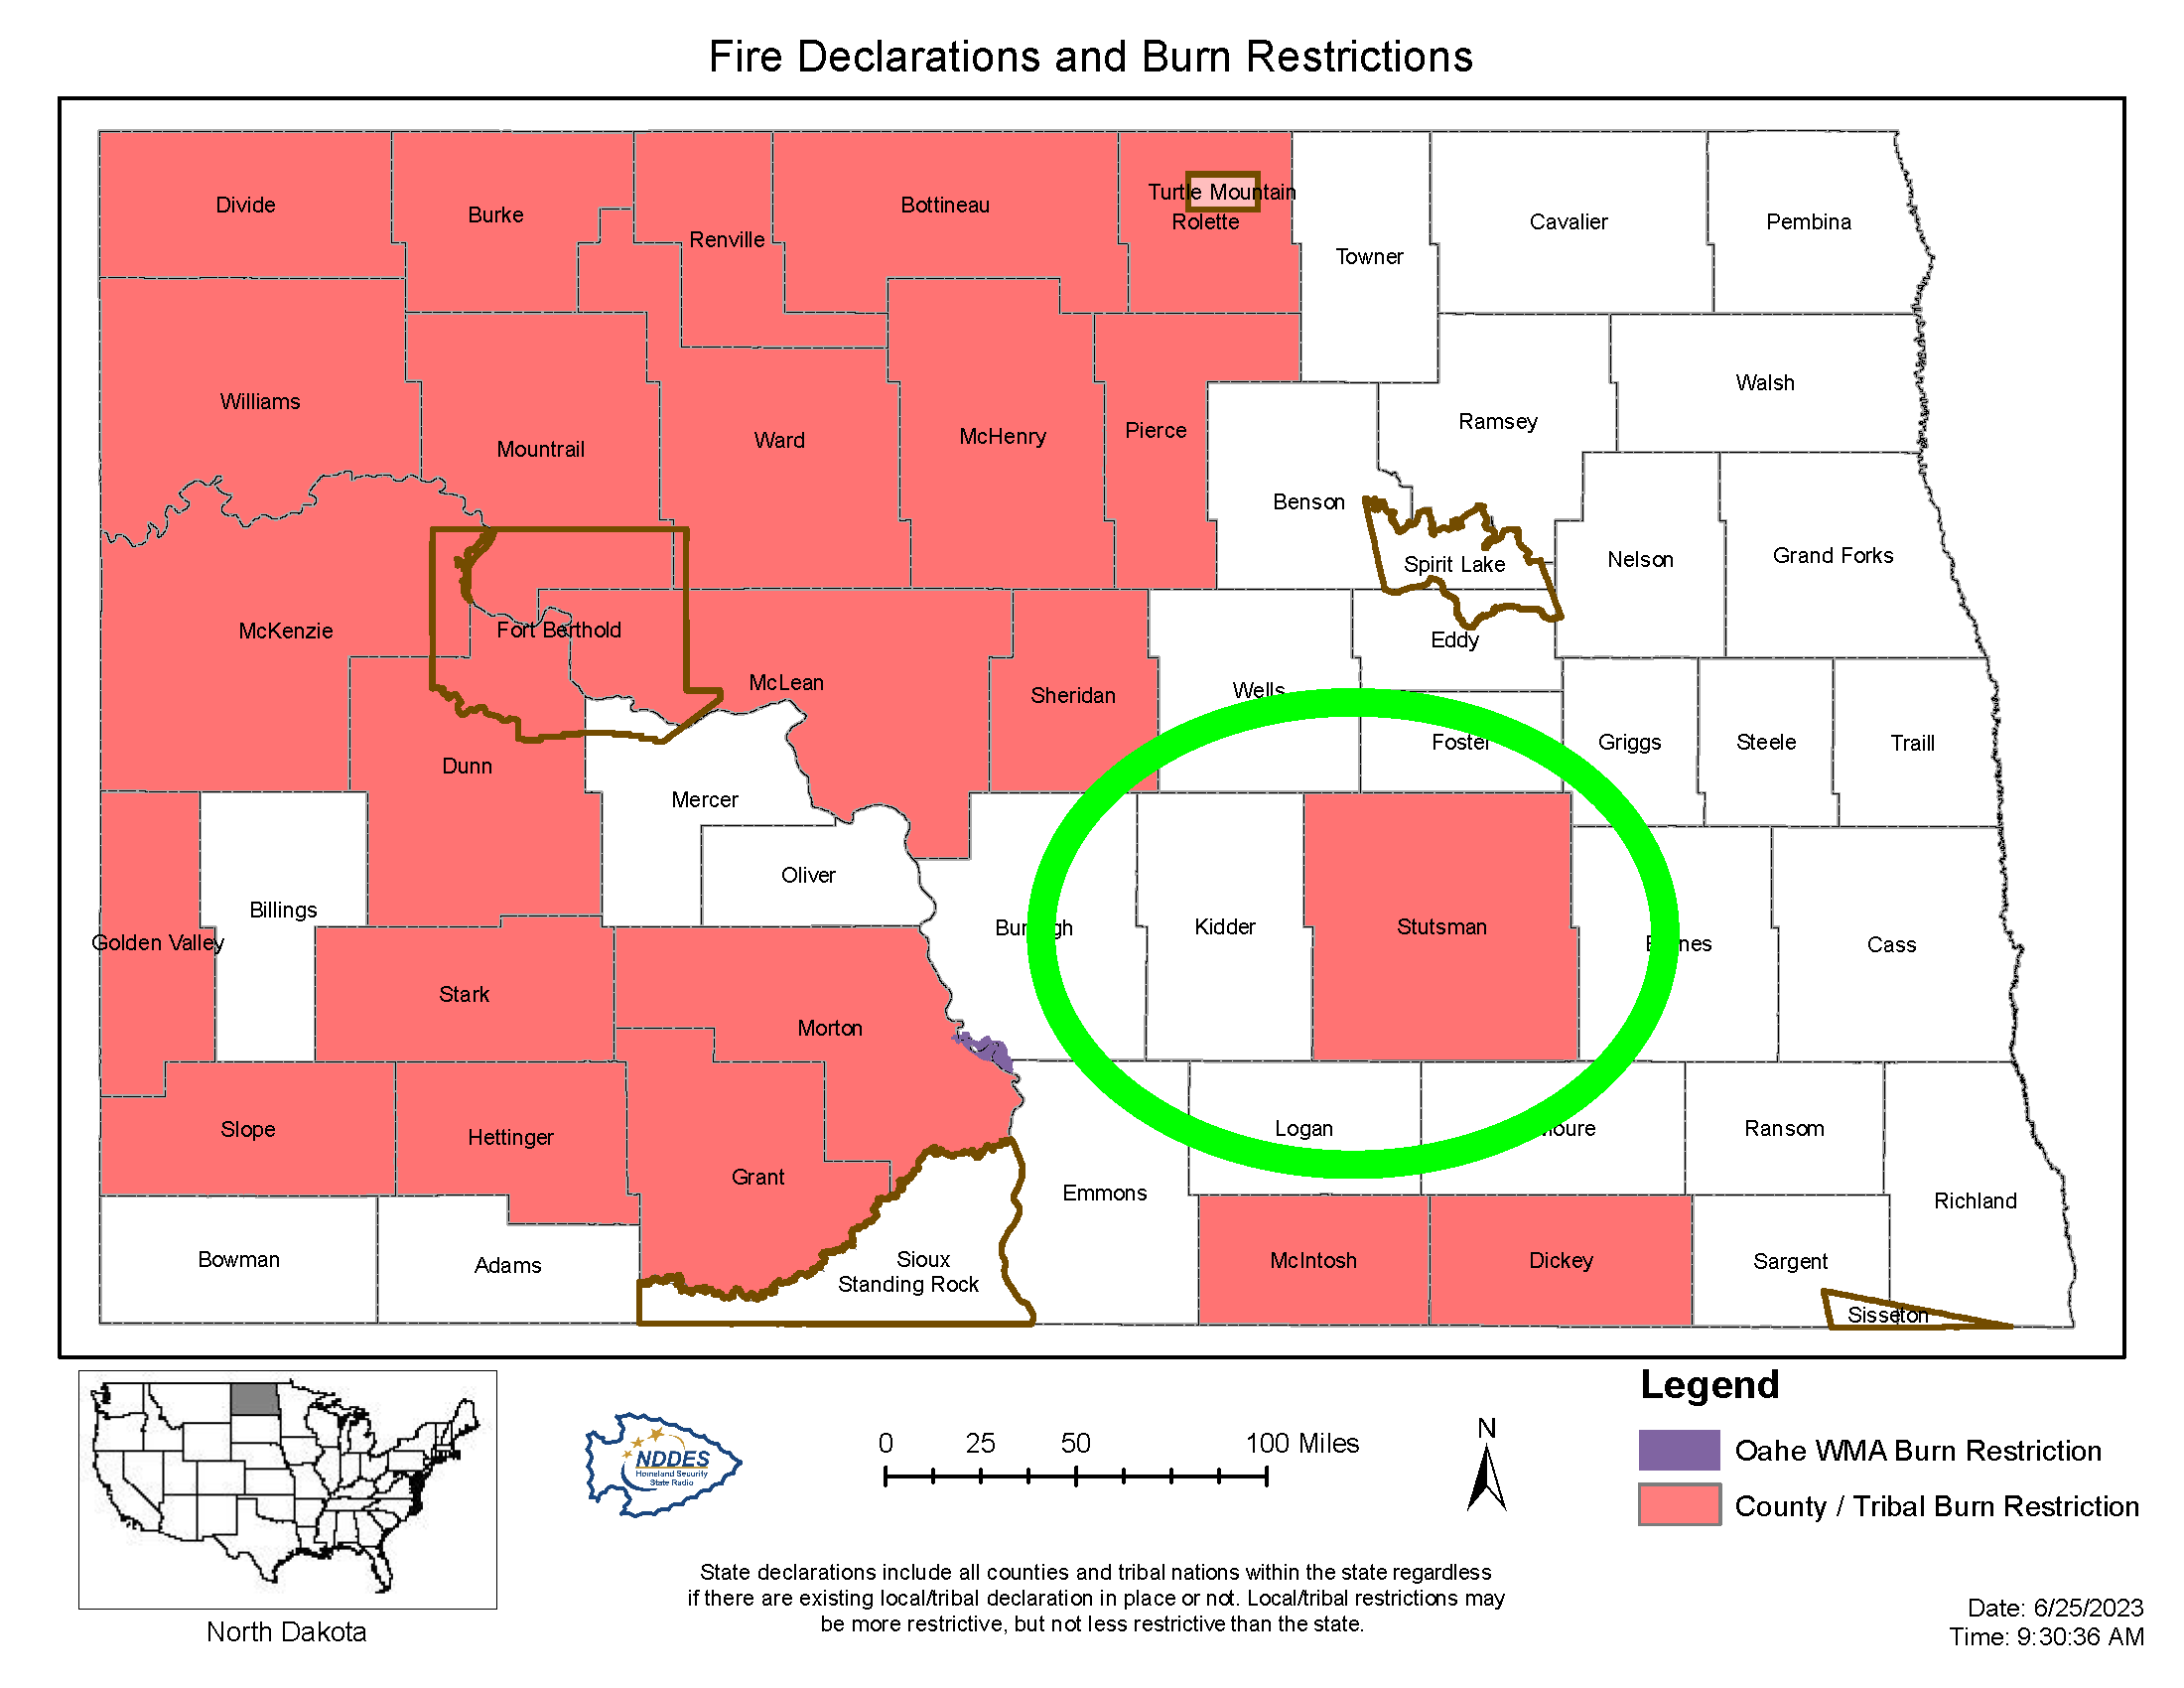
\includegraphics[width=1\linewidth]{figs/FireDeclarations.png} 
		\end{figure}
	\end{center}
\end{frame}

\begin{frame}{County-level burn restrictions}
	\begin{center}
		\begin{figure}
			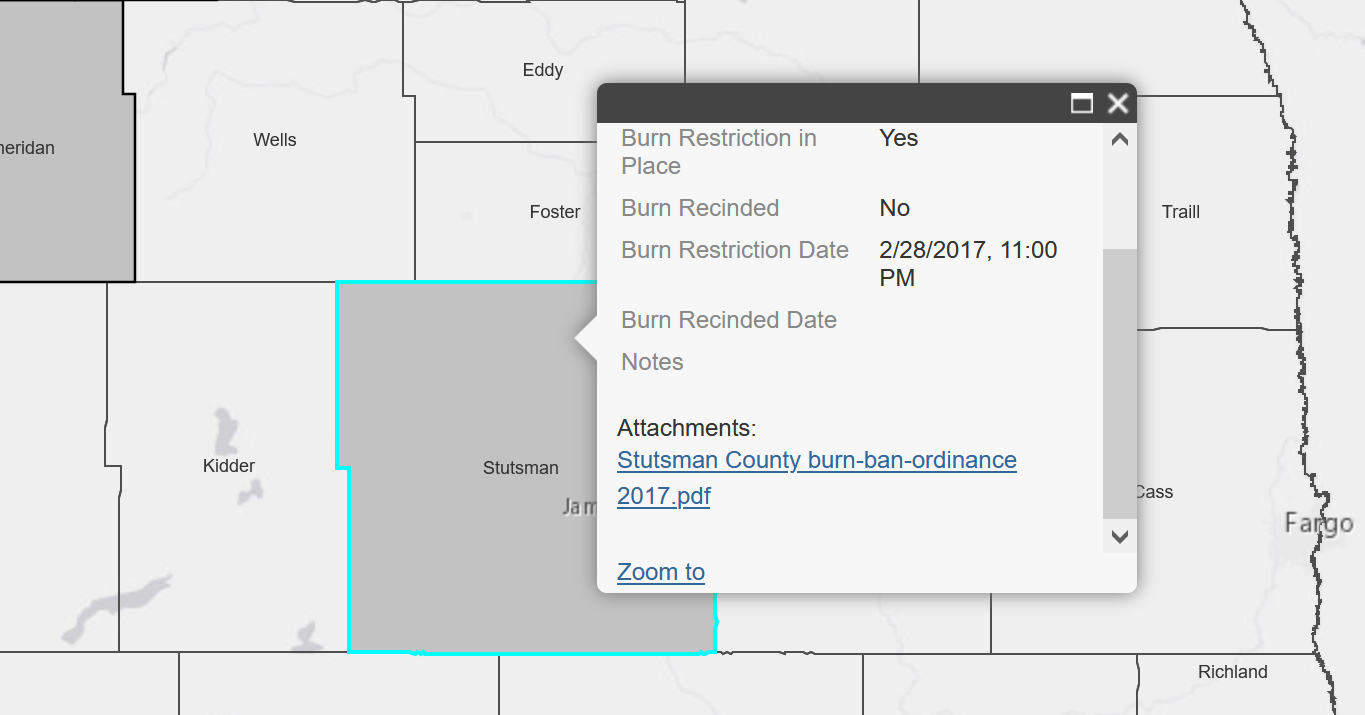
\includegraphics[width=1\linewidth]{figs/StutsmanBurnBan} 
		\end{figure}
	\end{center}
\end{frame}

\begin{frame}{Tying burn restrictions to real-time conditions}
	\begin{center}
		\begin{figure}
			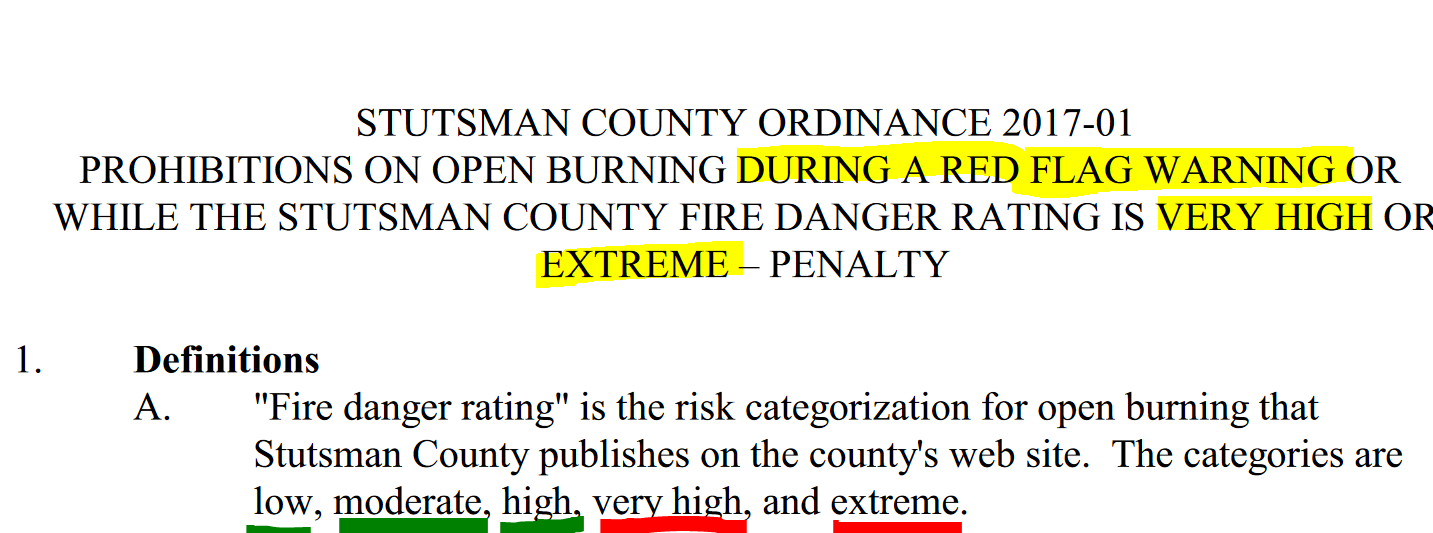
\includegraphics[width=1\linewidth]{figs/StutsmanOrdinance} 
		\end{figure}
	\end{center}
\end{frame}



\begin{frame}{Fire, grazing, and the pre-European landscape}
\alert{Pyric herbivory}
\begin{columns}
\begin{column}{0.5\textwidth}
\begin{itemize}
	\item Recent burns have high-quality forage
	\item[]
	\item Grazers focus on burned areas
	\item[]
	\item Vegetation grows up in other areas...
		\begin{itemize}
			\item providing habitat
			\item fueling future fires
		\end{itemize}
	\end{itemize}
\end{column}
\begin{column}{0.55\textwidth}  
\begin{center}
\begin{figure}
 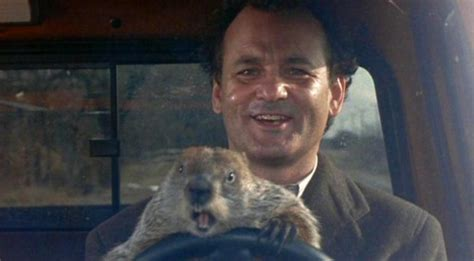
\includegraphics[width=1\linewidth]{figs/ghd} 
 
 \end{figure}
\end{center}
\end{column}
\end{columns}
\end{frame}



\begin{frame}{Disturbance-driven vs. inherent heterogeneity}
\begin{center}
\begin{figure}
 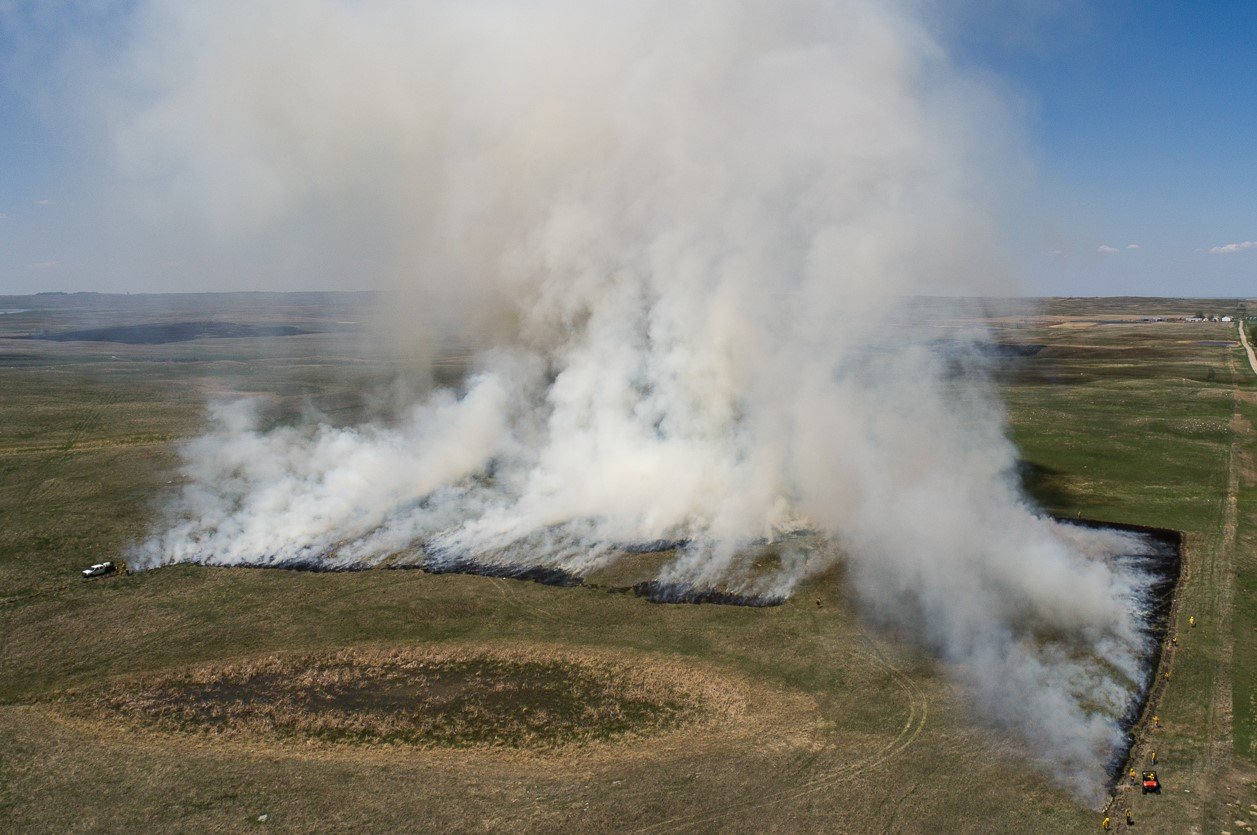
\includegraphics[width=1\linewidth]{figs/StreeterFire_17} 
 \end{figure}
\end{center}
\end{frame}



\begin{frame}{Testing PBG 2.0 in the Northern Great Plains } 
	\begin{columns}
		\begin{column}{0.6\textwidth}
			\begin{itemize}
				\item \alert{Streeter (Central Grasslands)}
				\begin{itemize}
					\item \textbf{Compares grazing systems}
					\item 4 pastures x 3 systems; cattle
					\item \emph{Poa pratensis}-invaded mixed-grass prairie
					\item 46 cm (18") annual rainfall
				\end{itemize}
				\item \alert{Hettinger}
				\begin{itemize}
					\item \textbf{Compares cattle \& sheep}
					\item 3 x cattle, 3 x sheep PBG
					\item Mostly non-native, cool-season grasses
					\item post-CRP pasture stands
					\item 40 cm (16") annual rainfall
				\end{itemize}
			\end{itemize}
		\end{column}
		\begin{column}{0.45\textwidth}  
			\begin{center}
				\begin{figure}
					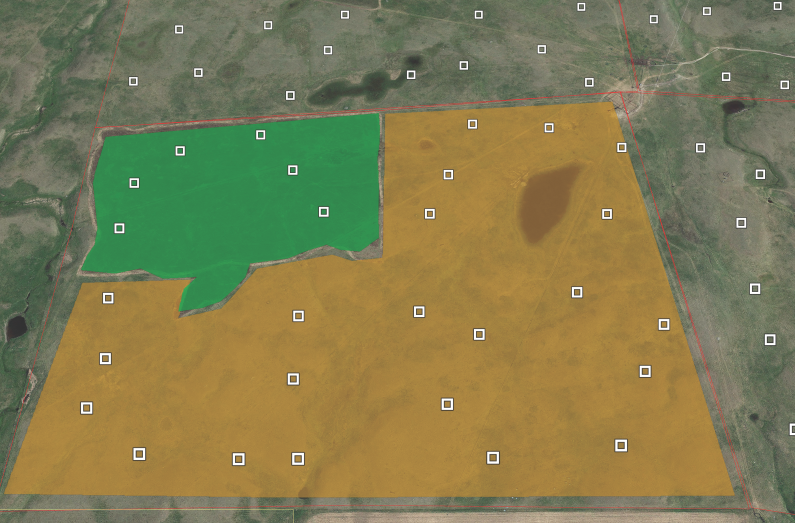
\includegraphics[width=1\linewidth]{figs/BobPasture}  
				\end{figure}
			\end{center}
		\end{column}
	\end{columns}
\end{frame}

\begin{frame}{Mopping up} 
\alert{Prescribed fire has direct benefits to livestock production}
\begin{columns}
\begin{column}{0.55\textwidth}
\begin{itemize}
	\item Livestock focus grazing in recently-burned patches
	\item[]
	\item Burned areas have better forage
	\item[]
	\item Fire has positive or neutral effects on soil
	\item[]
	\item Patch-burning enhances conservation outcomes, too
\end{itemize}
\end{column}
\begin{column}{0.5\textwidth}  
\begin{center}
\begin{figure}
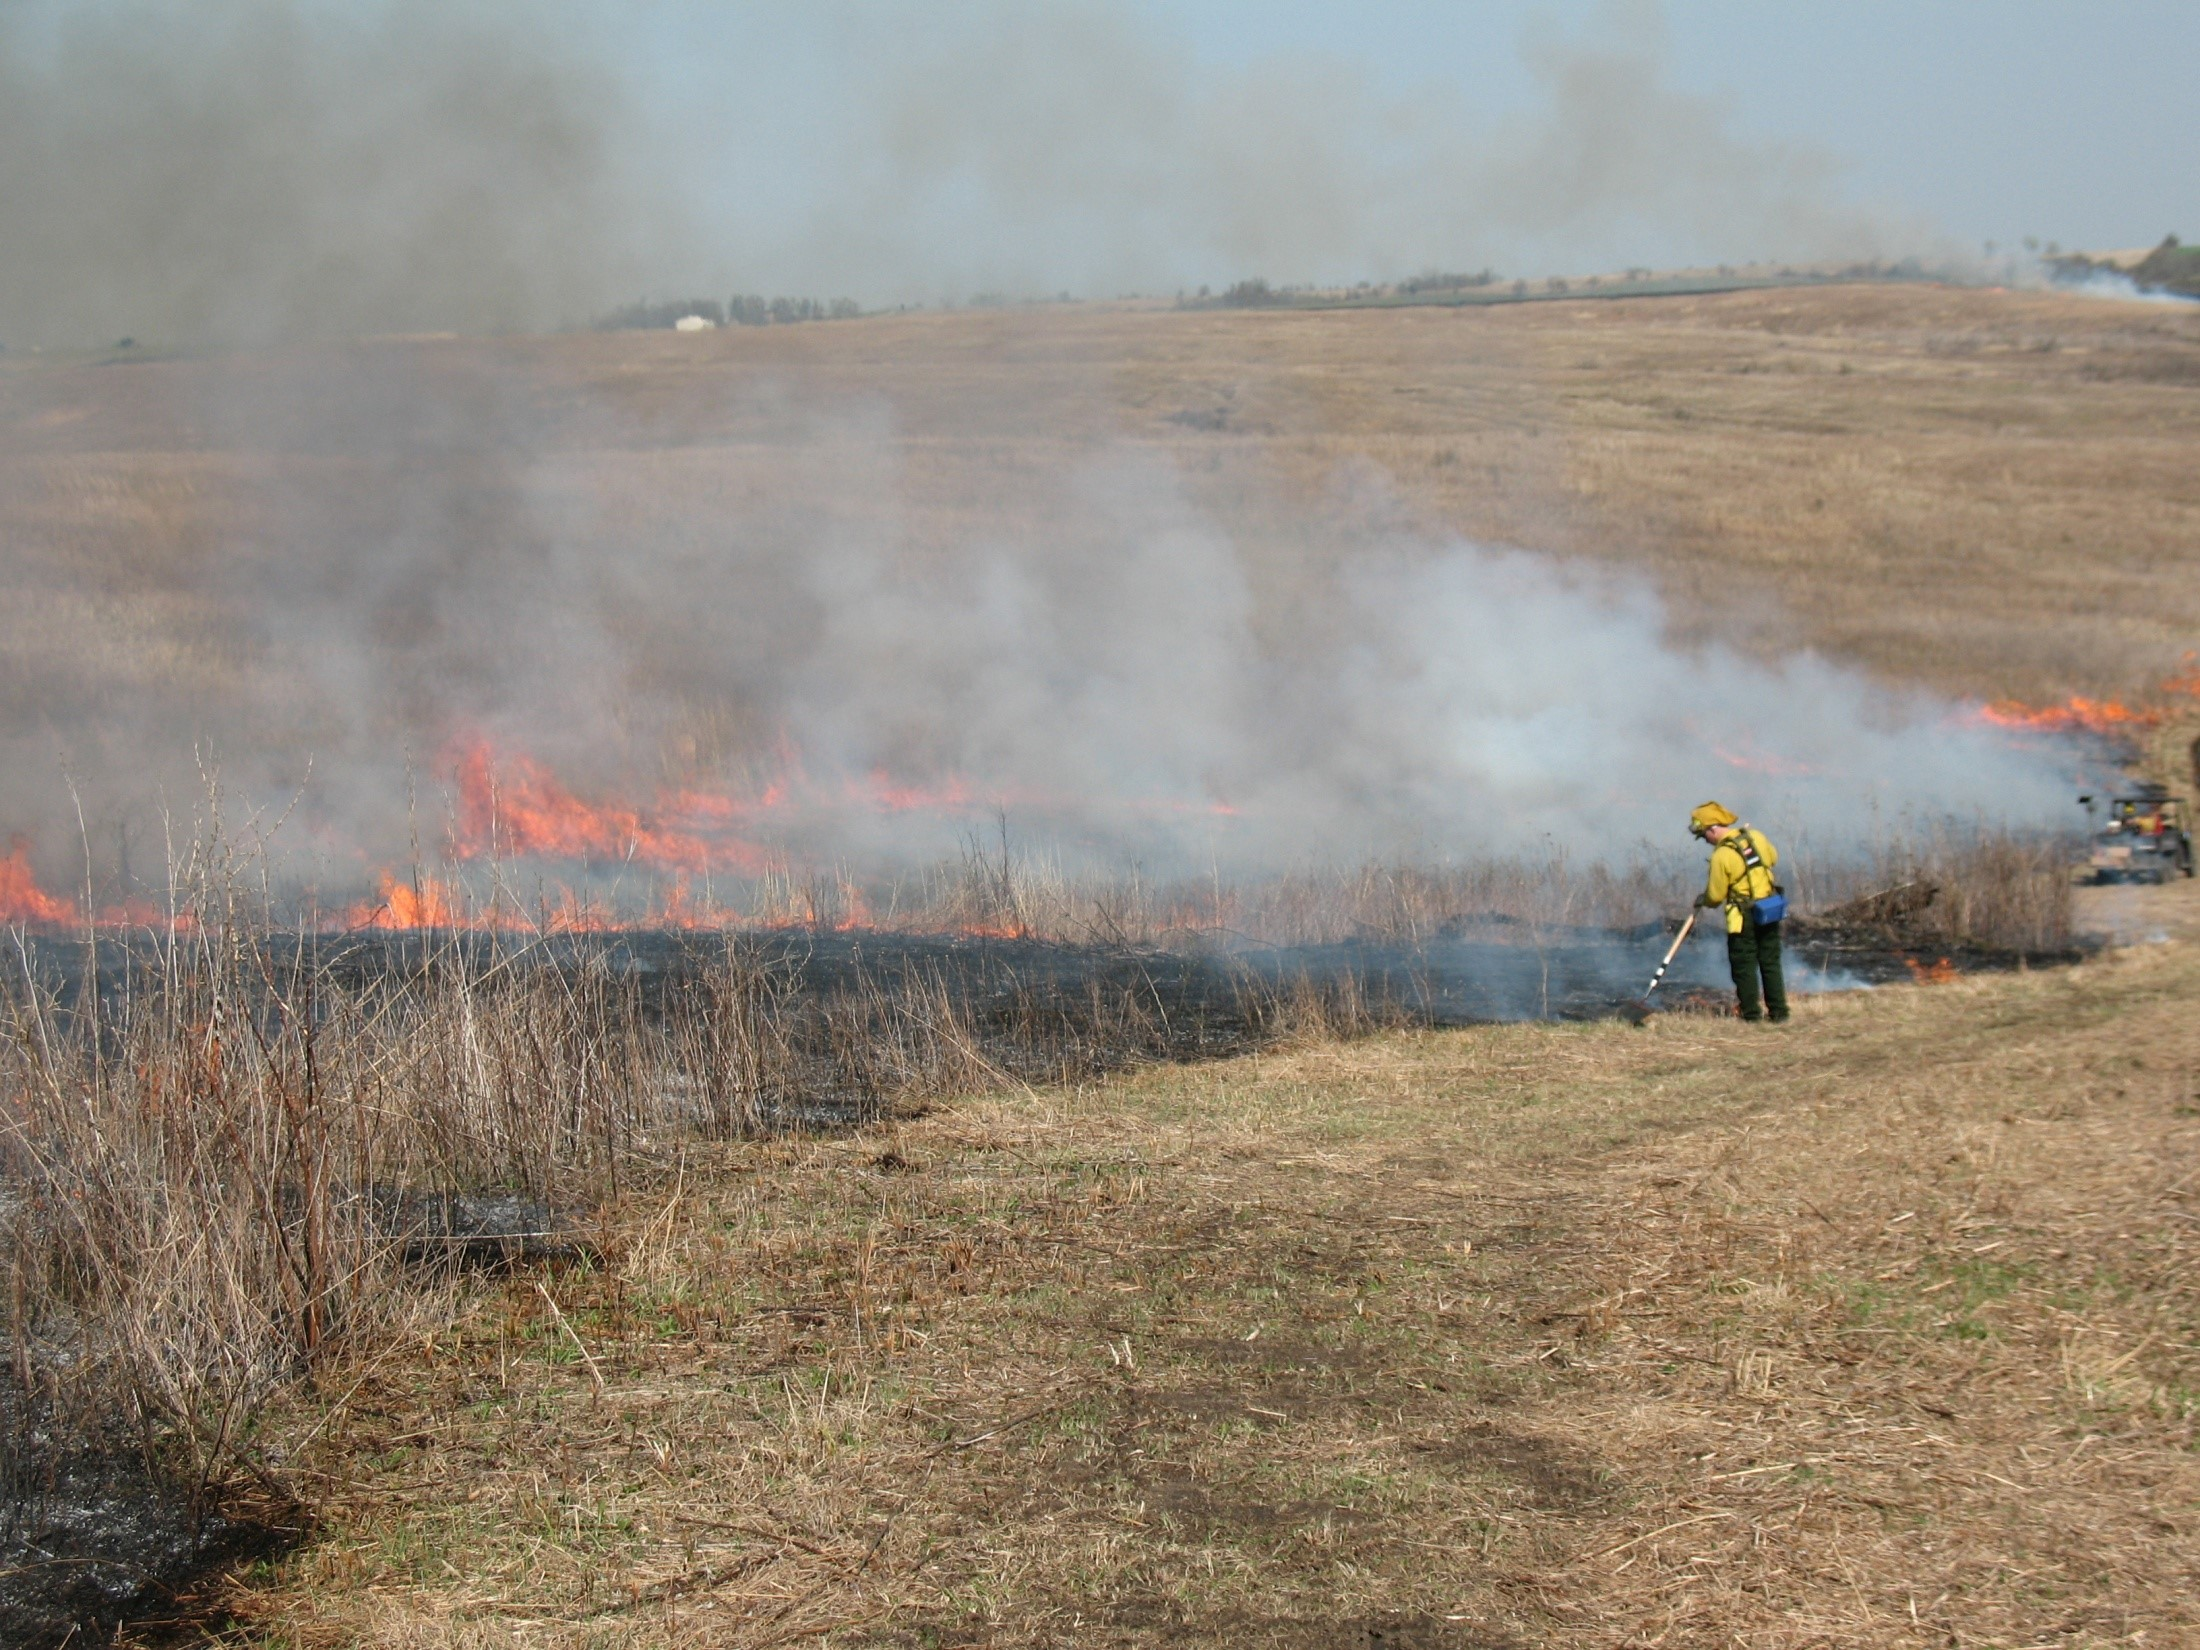
\includegraphics[width=1\linewidth]{figs/mop_up} 
 \end{figure}
\end{center}
\end{column}
\end{columns}
\end{frame}

\begin{frame}{Thank you!}
Any questions before you all run away?
\begin{center}
\begin{figure}
 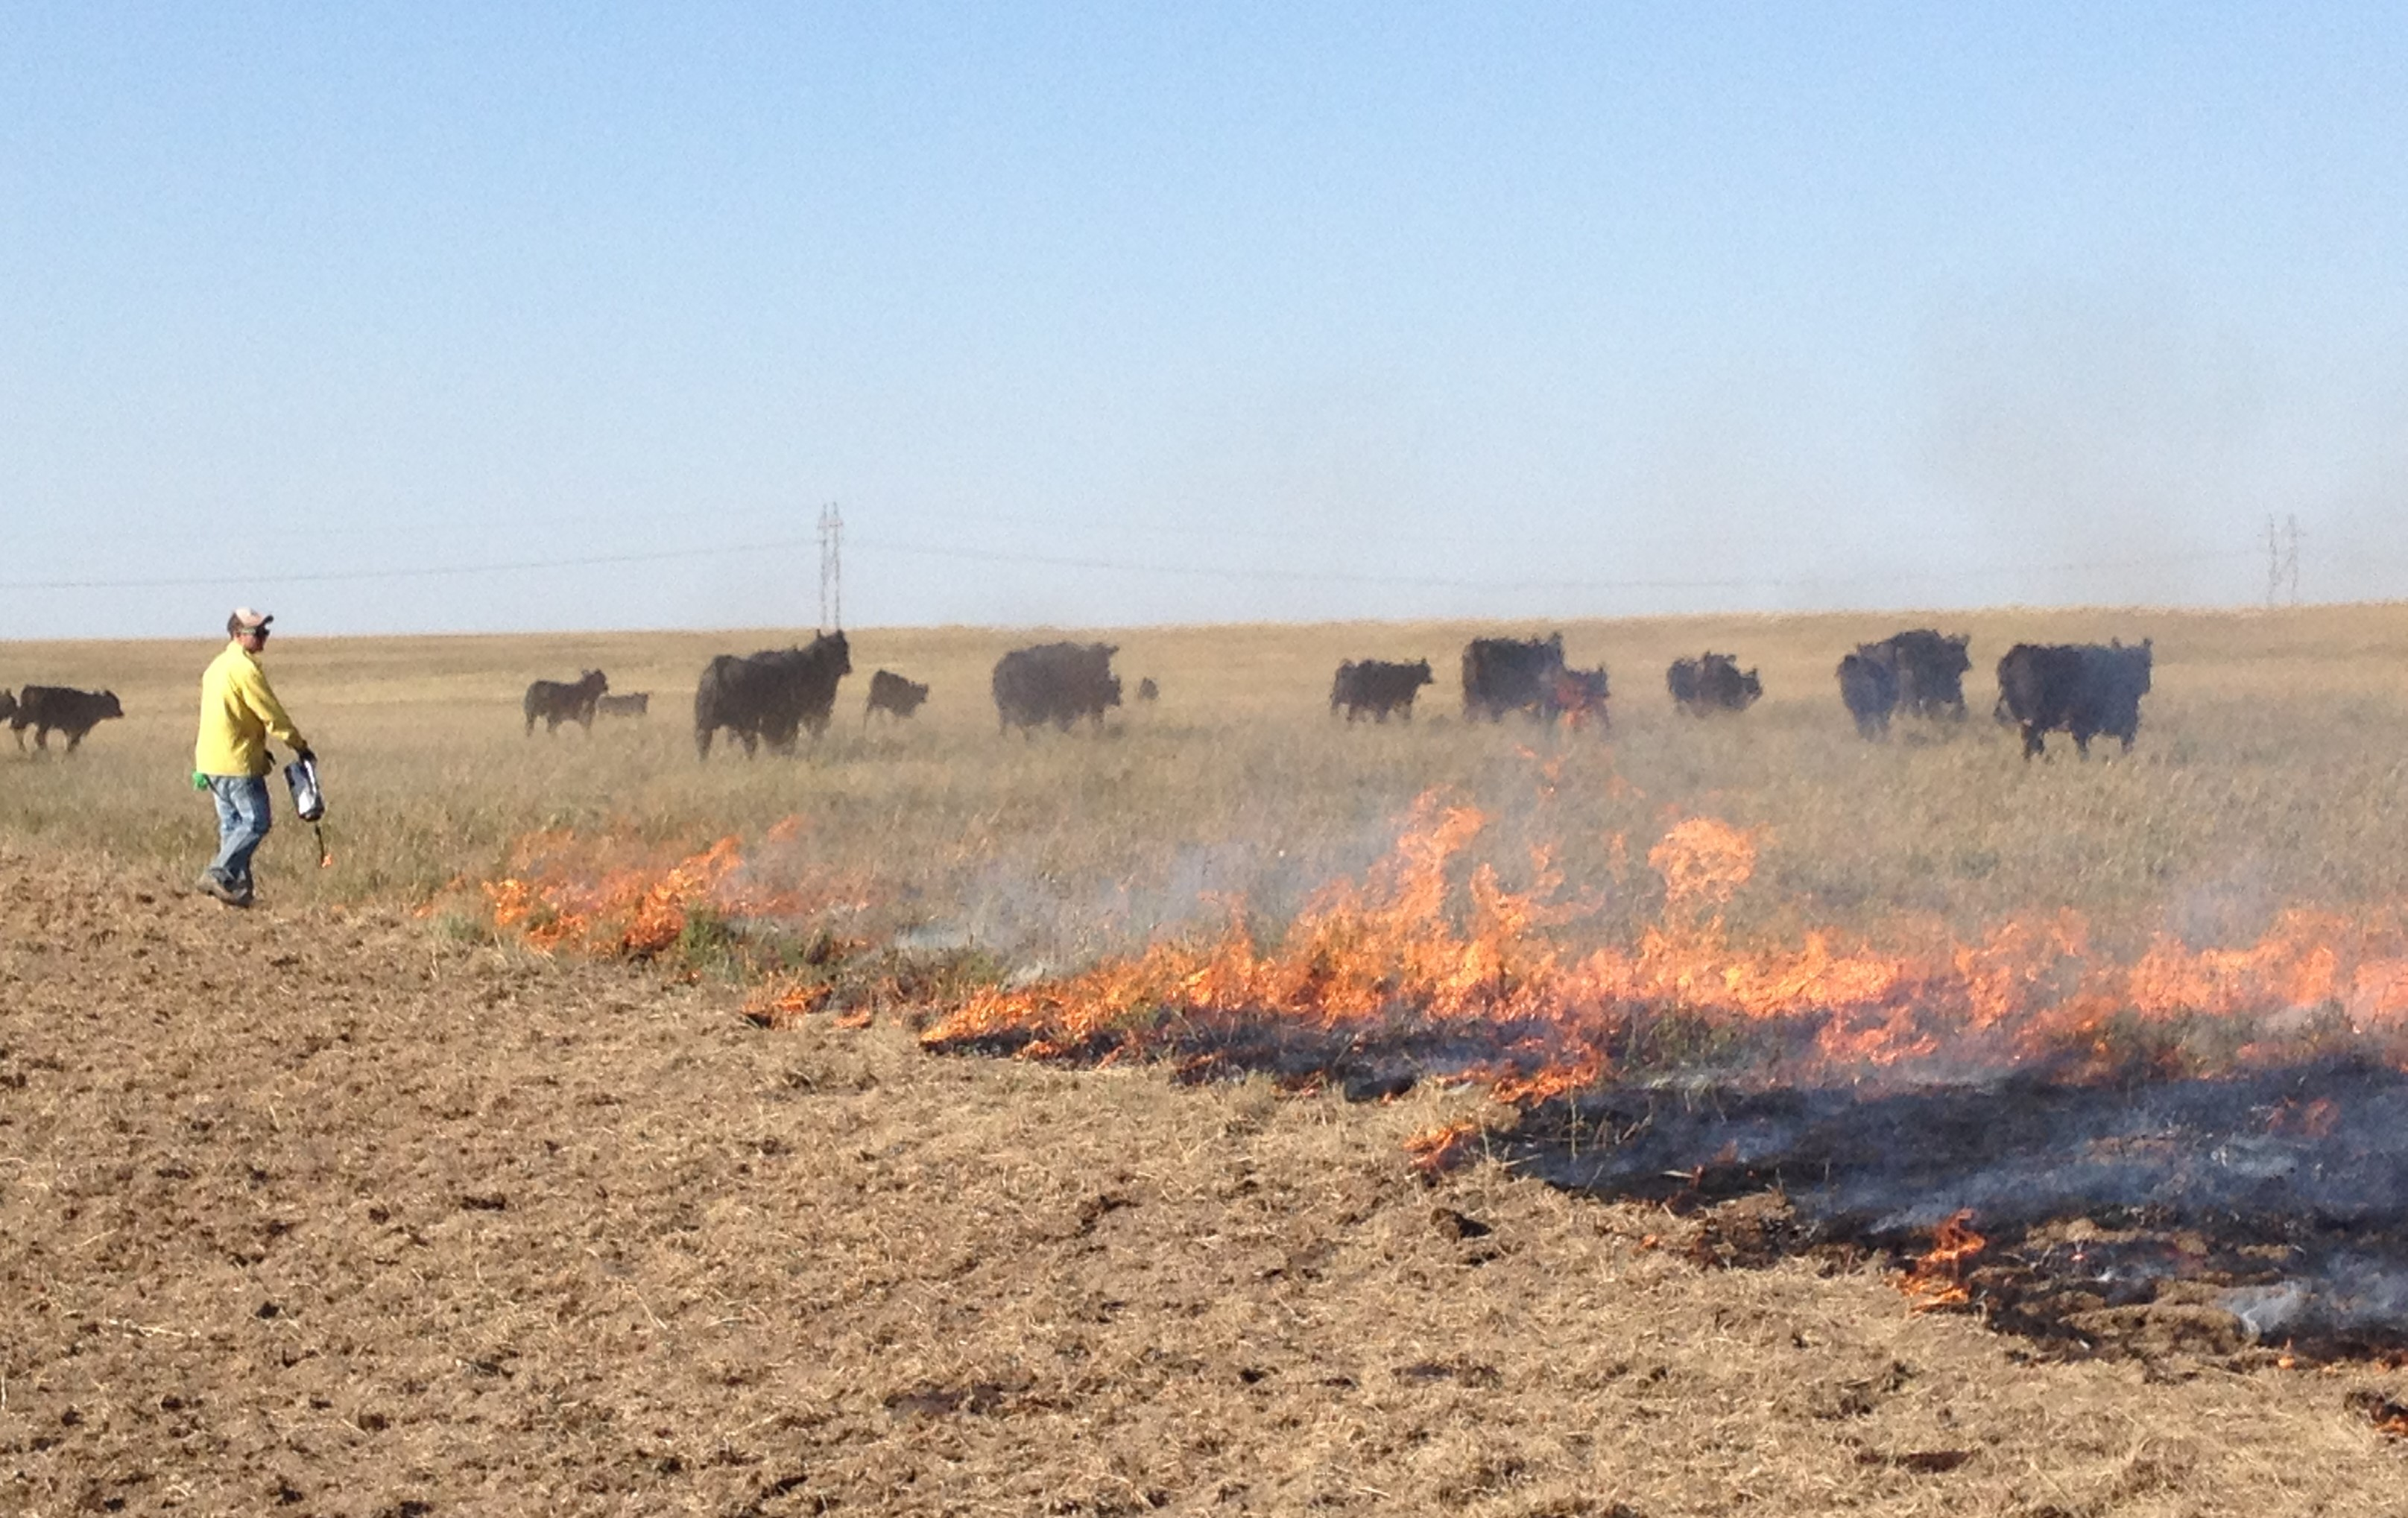
\includegraphics[width=1\linewidth]{figs/fire_cows_close} 

 \end{figure}
\end{center}
\end{frame}

\end{document}
